\begin{figure}[H] \centering % Created by tikzDevice version 0.12.4 on 2023-06-16 21:07:30
% !TEX encoding = UTF-8 Unicode
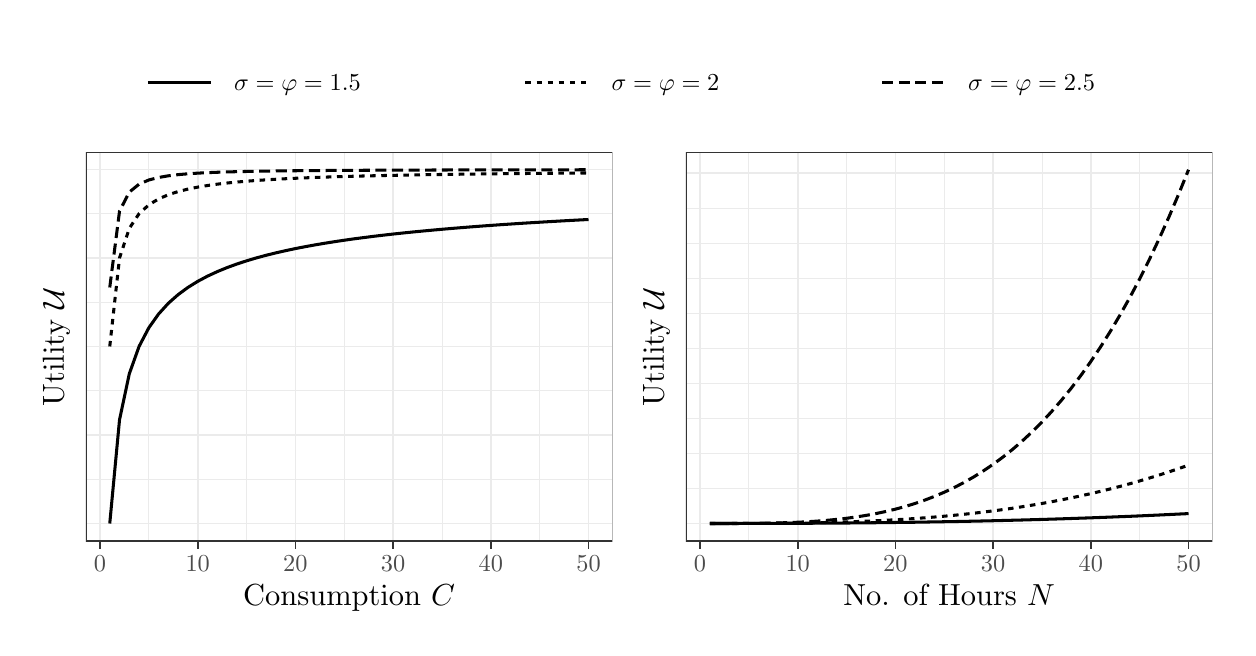
\begin{tikzpicture}[x=1pt,y=1pt]
\definecolor{fillColor}{RGB}{255,255,255}
\path[use as bounding box,fill=fillColor,fill opacity=0.00] (0,0) rectangle (433.62,216.81);
\begin{scope}
\path[clip] (  0.00,  0.00) rectangle (433.62,216.81);
\definecolor{fillColor}{RGB}{255,255,255}

\path[fill=fillColor] ( -8.70,177.36) rectangle (442.32,216.81);
\end{scope}

\begin{scope}
\path[clip] (  0.00,  0.00) rectangle (433.62,216.81);
\definecolor{fillColor}{RGB}{255,255,255}

\path[fill=fillColor] ( 40.62,182.86) rectangle ( 69.07,211.31);
\end{scope}
\begin{scope}
\path[clip] (  0.00,  0.00) rectangle (433.62,216.81);
\definecolor{drawColor}{RGB}{0,0,0}

\path[draw=drawColor,line width= 1.1pt,line join=round] ( 43.47,197.08) -- ( 66.23,197.08);
\end{scope}
\begin{scope}
\path[clip] (  0.00,  0.00) rectangle (433.62,216.81);
\definecolor{fillColor}{RGB}{255,255,255}

\path[fill=fillColor] (177.03,182.86) rectangle (205.49,211.31);
\end{scope}
\begin{scope}
\path[clip] (  0.00,  0.00) rectangle (433.62,216.81);
\definecolor{drawColor}{RGB}{0,0,0}

\path[draw=drawColor,line width= 1.1pt,dash pattern=on 2pt off 2pt ,line join=round] (179.88,197.08) -- (202.64,197.08);
\end{scope}
\begin{scope}
\path[clip] (  0.00,  0.00) rectangle (433.62,216.81);
\definecolor{fillColor}{RGB}{255,255,255}

\path[fill=fillColor] (305.91,182.86) rectangle (334.36,211.31);
\end{scope}
\begin{scope}
\path[clip] (  0.00,  0.00) rectangle (433.62,216.81);
\definecolor{drawColor}{RGB}{0,0,0}

\path[draw=drawColor,line width= 1.1pt,dash pattern=on 4pt off 2pt ,line join=round] (308.76,197.08) -- (331.52,197.08);
\end{scope}
\begin{scope}
\path[clip] (  0.00,  0.00) rectangle (433.62,216.81);
\definecolor{drawColor}{RGB}{0,0,0}

\node[text=drawColor,anchor=base west,inner sep=0pt, outer sep=0pt, scale=  0.88] at ( 74.57,194.05) {$\sigma = \varphi = 1.5$};
\end{scope}
\begin{scope}
\path[clip] (  0.00,  0.00) rectangle (433.62,216.81);
\definecolor{drawColor}{RGB}{0,0,0}

\node[text=drawColor,anchor=base west,inner sep=0pt, outer sep=0pt, scale=  0.88] at (210.99,194.05) {$\sigma = \varphi = 2$};
\end{scope}
\begin{scope}
\path[clip] (  0.00,  0.00) rectangle (433.62,216.81);
\definecolor{drawColor}{RGB}{0,0,0}

\node[text=drawColor,anchor=base west,inner sep=0pt, outer sep=0pt, scale=  0.88] at (339.86,194.05) {$\sigma = \varphi = 2.5$};
\end{scope}
\begin{scope}
\path[clip] (  0.00,  0.00) rectangle (216.81,177.36);
\definecolor{drawColor}{RGB}{255,255,255}
\definecolor{fillColor}{RGB}{255,255,255}

\path[draw=drawColor,line width= 0.6pt,line join=round,line cap=round,fill=fillColor] (  0.00,  0.00) rectangle (216.81,177.36);
\end{scope}
\begin{scope}
\path[clip] ( 21.01, 31.25) rectangle (211.31,171.86);
\definecolor{fillColor}{RGB}{255,255,255}

\path[fill=fillColor] ( 21.01, 31.25) rectangle (211.31,171.86);
\definecolor{drawColor}{gray}{0.92}

\path[draw=drawColor,line width= 0.3pt,line join=round] ( 21.01, 53.64) --
	(211.31, 53.64);

\path[draw=drawColor,line width= 0.3pt,line join=round] ( 21.01, 85.62) --
	(211.31, 85.62);

\path[draw=drawColor,line width= 0.3pt,line join=round] ( 21.01,117.61) --
	(211.31,117.61);

\path[draw=drawColor,line width= 0.3pt,line join=round] ( 21.01,149.59) --
	(211.31,149.59);

\path[draw=drawColor,line width= 0.3pt,line join=round] ( 43.78, 31.25) --
	( 43.78,171.86);

\path[draw=drawColor,line width= 0.3pt,line join=round] ( 79.09, 31.25) --
	( 79.09,171.86);

\path[draw=drawColor,line width= 0.3pt,line join=round] (114.39, 31.25) --
	(114.39,171.86);

\path[draw=drawColor,line width= 0.3pt,line join=round] (149.70, 31.25) --
	(149.70,171.86);

\path[draw=drawColor,line width= 0.3pt,line join=round] (185.01, 31.25) --
	(185.01,171.86);

\path[draw=drawColor,line width= 0.6pt,line join=round] ( 21.01, 37.64) --
	(211.31, 37.64);

\path[draw=drawColor,line width= 0.6pt,line join=round] ( 21.01, 69.63) --
	(211.31, 69.63);

\path[draw=drawColor,line width= 0.6pt,line join=round] ( 21.01,101.62) --
	(211.31,101.62);

\path[draw=drawColor,line width= 0.6pt,line join=round] ( 21.01,133.60) --
	(211.31,133.60);

\path[draw=drawColor,line width= 0.6pt,line join=round] ( 21.01,165.59) --
	(211.31,165.59);

\path[draw=drawColor,line width= 0.6pt,line join=round] ( 26.12, 31.25) --
	( 26.12,171.86);

\path[draw=drawColor,line width= 0.6pt,line join=round] ( 61.43, 31.25) --
	( 61.43,171.86);

\path[draw=drawColor,line width= 0.6pt,line join=round] ( 96.74, 31.25) --
	( 96.74,171.86);

\path[draw=drawColor,line width= 0.6pt,line join=round] (132.05, 31.25) --
	(132.05,171.86);

\path[draw=drawColor,line width= 0.6pt,line join=round] (167.35, 31.25) --
	(167.35,171.86);

\path[draw=drawColor,line width= 0.6pt,line join=round] (202.66, 31.25) --
	(202.66,171.86);
\definecolor{drawColor}{RGB}{0,0,0}

\path[draw=drawColor,line width= 1.1pt,line join=round] ( 29.66, 37.64) --
	( 33.19, 75.12) --
	( 36.72, 91.72) --
	( 40.25,101.62) --
	( 43.78,108.37) --
	( 47.31,113.35) --
	( 50.84,117.23) --
	( 54.37,120.35) --
	( 57.90,122.94) --
	( 61.43,125.13) --
	( 64.96,127.01) --
	( 68.49,128.65) --
	( 72.02,130.10) --
	( 75.55,131.39) --
	( 79.09,132.55) --
	( 82.62,133.60) --
	( 86.15,134.56) --
	( 89.68,135.43) --
	( 93.21,136.23) --
	( 96.74,136.98) --
	(100.27,137.67) --
	(103.80,138.31) --
	(107.33,138.91) --
	(110.86,139.47) --
	(114.39,140.00) --
	(117.92,140.50) --
	(121.45,140.96) --
	(124.98,141.41) --
	(128.51,141.83) --
	(132.05,142.23) --
	(135.58,142.61) --
	(139.11,142.97) --
	(142.64,143.31) --
	(146.17,143.64) --
	(149.70,143.96) --
	(153.23,144.26) --
	(156.76,144.55) --
	(160.29,144.83) --
	(163.82,145.10) --
	(167.35,145.36) --
	(170.88,145.61) --
	(174.41,145.84) --
	(177.94,146.08) --
	(181.48,146.30) --
	(185.01,146.51) --
	(188.54,146.72) --
	(192.07,146.92) --
	(195.60,147.12) --
	(199.13,147.31) --
	(202.66,147.49);

\path[draw=drawColor,line width= 1.1pt,dash pattern=on 2pt off 2pt ,line join=round] ( 29.66,101.62) --
	( 33.19,133.60) --
	( 36.72,144.26) --
	( 40.25,149.59) --
	( 43.78,152.79) --
	( 47.31,154.92) --
	( 50.84,156.45) --
	( 54.37,157.59) --
	( 57.90,158.48) --
	( 61.43,159.19) --
	( 64.96,159.77) --
	( 68.49,160.26) --
	( 72.02,160.67) --
	( 75.55,161.02) --
	( 79.09,161.32) --
	( 82.62,161.59) --
	( 86.15,161.82) --
	( 89.68,162.03) --
	( 93.21,162.22) --
	( 96.74,162.39) --
	(100.27,162.54) --
	(103.80,162.68) --
	(107.33,162.81) --
	(110.86,162.92) --
	(114.39,163.03) --
	(117.92,163.13) --
	(121.45,163.22) --
	(124.98,163.30) --
	(128.51,163.38) --
	(132.05,163.45) --
	(135.58,163.52) --
	(139.11,163.59) --
	(142.64,163.65) --
	(146.17,163.71) --
	(149.70,163.76) --
	(153.23,163.81) --
	(156.76,163.86) --
	(160.29,163.90) --
	(163.82,163.95) --
	(167.35,163.99) --
	(170.88,164.03) --
	(174.41,164.06) --
	(177.94,164.10) --
	(181.48,164.13) --
	(185.01,164.17) --
	(188.54,164.20) --
	(192.07,164.23) --
	(195.60,164.25) --
	(199.13,164.28) --
	(202.66,164.31);

\path[draw=drawColor,line width= 1.1pt,dash pattern=on 4pt off 2pt ,line join=round] ( 29.66,122.94) --
	( 33.19,150.51) --
	( 36.72,157.38) --
	( 40.25,160.26) --
	( 43.78,161.77) --
	( 47.31,162.68) --
	( 50.84,163.28) --
	( 54.37,163.70) --
	( 57.90,164.01) --
	( 61.43,164.24) --
	( 64.96,164.42) --
	( 68.49,164.56) --
	( 72.02,164.68) --
	( 75.55,164.77) --
	( 79.09,164.85) --
	( 82.62,164.92) --
	( 86.15,164.98) --
	( 89.68,165.03) --
	( 93.21,165.07) --
	( 96.74,165.11) --
	(100.27,165.14) --
	(103.80,165.17) --
	(107.33,165.20) --
	(110.86,165.22) --
	(114.39,165.25) --
	(117.92,165.27) --
	(121.45,165.28) --
	(124.98,165.30) --
	(128.51,165.31) --
	(132.05,165.33) --
	(135.58,165.34) --
	(139.11,165.35) --
	(142.64,165.36) --
	(146.17,165.37) --
	(149.70,165.38) --
	(153.23,165.39) --
	(156.76,165.40) --
	(160.29,165.40) --
	(163.82,165.41) --
	(167.35,165.42) --
	(170.88,165.42) --
	(174.41,165.43) --
	(177.94,165.44) --
	(181.48,165.44) --
	(185.01,165.45) --
	(188.54,165.45) --
	(192.07,165.45) --
	(195.60,165.46) --
	(199.13,165.46) --
	(202.66,165.47);
\definecolor{drawColor}{gray}{0.20}

\path[draw=drawColor,line width= 0.6pt,line join=round,line cap=round] ( 21.01, 31.25) rectangle (211.31,171.86);
\end{scope}
\begin{scope}
\path[clip] (  0.00,  0.00) rectangle (433.62,216.81);
\definecolor{drawColor}{gray}{0.20}

\path[draw=drawColor,line width= 0.6pt,line join=round] ( 26.12, 28.50) --
	( 26.12, 31.25);

\path[draw=drawColor,line width= 0.6pt,line join=round] ( 61.43, 28.50) --
	( 61.43, 31.25);

\path[draw=drawColor,line width= 0.6pt,line join=round] ( 96.74, 28.50) --
	( 96.74, 31.25);

\path[draw=drawColor,line width= 0.6pt,line join=round] (132.05, 28.50) --
	(132.05, 31.25);

\path[draw=drawColor,line width= 0.6pt,line join=round] (167.35, 28.50) --
	(167.35, 31.25);

\path[draw=drawColor,line width= 0.6pt,line join=round] (202.66, 28.50) --
	(202.66, 31.25);
\end{scope}
\begin{scope}
\path[clip] (  0.00,  0.00) rectangle (433.62,216.81);
\definecolor{drawColor}{gray}{0.30}

\node[text=drawColor,anchor=base,inner sep=0pt, outer sep=0pt, scale=  0.88] at ( 26.12, 20.24) {0};

\node[text=drawColor,anchor=base,inner sep=0pt, outer sep=0pt, scale=  0.88] at ( 61.43, 20.24) {10};

\node[text=drawColor,anchor=base,inner sep=0pt, outer sep=0pt, scale=  0.88] at ( 96.74, 20.24) {20};

\node[text=drawColor,anchor=base,inner sep=0pt, outer sep=0pt, scale=  0.88] at (132.05, 20.24) {30};

\node[text=drawColor,anchor=base,inner sep=0pt, outer sep=0pt, scale=  0.88] at (167.35, 20.24) {40};

\node[text=drawColor,anchor=base,inner sep=0pt, outer sep=0pt, scale=  0.88] at (202.66, 20.24) {50};
\end{scope}
\begin{scope}
\path[clip] (  0.00,  0.00) rectangle (433.62,216.81);
\definecolor{drawColor}{RGB}{0,0,0}

\node[text=drawColor,anchor=base,inner sep=0pt, outer sep=0pt, scale=  1.10] at (116.16,  7.93) {Consumption $C$};
\end{scope}
\begin{scope}
\path[clip] (  0.00,  0.00) rectangle (433.62,216.81);
\definecolor{drawColor}{RGB}{0,0,0}

\node[text=drawColor,rotate= 90.00,anchor=base,inner sep=0pt, outer sep=0pt, scale=  1.10] at ( 13.08,101.56) {Utility $\mathcal{U}$};
\end{scope}
\begin{scope}
\path[clip] (216.81,  0.00) rectangle (433.62,177.36);
\definecolor{drawColor}{RGB}{255,255,255}
\definecolor{fillColor}{RGB}{255,255,255}

\path[draw=drawColor,line width= 0.6pt,line join=round,line cap=round,fill=fillColor] (216.81,  0.00) rectangle (433.62,177.36);
\end{scope}
\begin{scope}
\path[clip] (237.82, 31.25) rectangle (428.12,171.86);
\definecolor{fillColor}{RGB}{255,255,255}

\path[fill=fillColor] (237.82, 31.25) rectangle (428.12,171.86);
\definecolor{drawColor}{gray}{0.92}

\path[draw=drawColor,line width= 0.3pt,line join=round] (237.82, 50.30) --
	(428.12, 50.30);

\path[draw=drawColor,line width= 0.3pt,line join=round] (237.82, 75.61) --
	(428.12, 75.61);

\path[draw=drawColor,line width= 0.3pt,line join=round] (237.82,100.91) --
	(428.12,100.91);

\path[draw=drawColor,line width= 0.3pt,line join=round] (237.82,126.22) --
	(428.12,126.22);

\path[draw=drawColor,line width= 0.3pt,line join=round] (237.82,151.53) --
	(428.12,151.53);

\path[draw=drawColor,line width= 0.3pt,line join=round] (260.59, 31.25) --
	(260.59,171.86);

\path[draw=drawColor,line width= 0.3pt,line join=round] (295.90, 31.25) --
	(295.90,171.86);

\path[draw=drawColor,line width= 0.3pt,line join=round] (331.20, 31.25) --
	(331.20,171.86);

\path[draw=drawColor,line width= 0.3pt,line join=round] (366.51, 31.25) --
	(366.51,171.86);

\path[draw=drawColor,line width= 0.3pt,line join=round] (401.82, 31.25) --
	(401.82,171.86);

\path[draw=drawColor,line width= 0.6pt,line join=round] (237.82, 37.64) --
	(428.12, 37.64);

\path[draw=drawColor,line width= 0.6pt,line join=round] (237.82, 62.95) --
	(428.12, 62.95);

\path[draw=drawColor,line width= 0.6pt,line join=round] (237.82, 88.26) --
	(428.12, 88.26);

\path[draw=drawColor,line width= 0.6pt,line join=round] (237.82,113.57) --
	(428.12,113.57);

\path[draw=drawColor,line width= 0.6pt,line join=round] (237.82,138.87) --
	(428.12,138.87);

\path[draw=drawColor,line width= 0.6pt,line join=round] (237.82,164.18) --
	(428.12,164.18);

\path[draw=drawColor,line width= 0.6pt,line join=round] (242.93, 31.25) --
	(242.93,171.86);

\path[draw=drawColor,line width= 0.6pt,line join=round] (278.24, 31.25) --
	(278.24,171.86);

\path[draw=drawColor,line width= 0.6pt,line join=round] (313.55, 31.25) --
	(313.55,171.86);

\path[draw=drawColor,line width= 0.6pt,line join=round] (348.86, 31.25) --
	(348.86,171.86);

\path[draw=drawColor,line width= 0.6pt,line join=round] (384.16, 31.25) --
	(384.16,171.86);

\path[draw=drawColor,line width= 0.6pt,line join=round] (419.47, 31.25) --
	(419.47,171.86);
\definecolor{drawColor}{RGB}{0,0,0}

\path[draw=drawColor,line width= 1.1pt,line join=round] (246.47, 37.64) --
	(250.00, 37.65) --
	(253.53, 37.65) --
	(257.06, 37.65) --
	(260.59, 37.66) --
	(264.12, 37.66) --
	(267.65, 37.67) --
	(271.18, 37.68) --
	(274.71, 37.69) --
	(278.24, 37.71) --
	(281.77, 37.73) --
	(285.30, 37.75) --
	(288.83, 37.77) --
	(292.36, 37.79) --
	(295.90, 37.82) --
	(299.43, 37.85) --
	(302.96, 37.89) --
	(306.49, 37.92) --
	(310.02, 37.96) --
	(313.55, 38.01) --
	(317.08, 38.05) --
	(320.61, 38.10) --
	(324.14, 38.16) --
	(327.67, 38.22) --
	(331.20, 38.28) --
	(334.73, 38.34) --
	(338.26, 38.41) --
	(341.79, 38.48) --
	(345.32, 38.56) --
	(348.86, 38.64) --
	(352.39, 38.73) --
	(355.92, 38.82) --
	(359.45, 38.91) --
	(362.98, 39.01) --
	(366.51, 39.11) --
	(370.04, 39.22) --
	(373.57, 39.33) --
	(377.10, 39.45) --
	(380.63, 39.57) --
	(384.16, 39.69) --
	(387.69, 39.82) --
	(391.22, 39.96) --
	(394.75, 40.10) --
	(398.29, 40.24) --
	(401.82, 40.39) --
	(405.35, 40.55) --
	(408.88, 40.71) --
	(412.41, 40.88) --
	(415.94, 41.05) --
	(419.47, 41.22);

\path[draw=drawColor,line width= 1.1pt,dash pattern=on 2pt off 2pt ,line join=round] (246.47, 37.64) --
	(250.00, 37.65) --
	(253.53, 37.65) --
	(257.06, 37.65) --
	(260.59, 37.67) --
	(264.12, 37.68) --
	(267.65, 37.70) --
	(271.18, 37.73) --
	(274.71, 37.77) --
	(278.24, 37.81) --
	(281.77, 37.87) --
	(285.30, 37.94) --
	(288.83, 38.01) --
	(292.36, 38.11) --
	(295.90, 38.21) --
	(299.43, 38.34) --
	(302.96, 38.47) --
	(306.49, 38.63) --
	(310.02, 38.80) --
	(313.55, 38.99) --
	(317.08, 39.21) --
	(320.61, 39.44) --
	(324.14, 39.70) --
	(327.67, 39.98) --
	(331.20, 40.28) --
	(334.73, 40.61) --
	(338.26, 40.97) --
	(341.79, 41.35) --
	(345.32, 41.76) --
	(348.86, 42.20) --
	(352.39, 42.67) --
	(355.92, 43.17) --
	(359.45, 43.71) --
	(362.98, 44.28) --
	(366.51, 44.88) --
	(370.04, 45.52) --
	(373.57, 46.19) --
	(377.10, 46.90) --
	(380.63, 47.65) --
	(384.16, 48.44) --
	(387.69, 49.27) --
	(391.22, 50.14) --
	(394.75, 51.06) --
	(398.29, 52.02) --
	(401.82, 53.02) --
	(405.35, 54.07) --
	(408.88, 55.16) --
	(412.41, 56.30) --
	(415.94, 57.49) --
	(419.47, 58.73);

\path[draw=drawColor,line width= 1.1pt,dash pattern=on 4pt off 2pt ,line join=round] (246.47, 37.64) --
	(250.00, 37.65) --
	(253.53, 37.65) --
	(257.06, 37.66) --
	(260.59, 37.68) --
	(264.12, 37.72) --
	(267.65, 37.78) --
	(271.18, 37.85) --
	(274.71, 37.96) --
	(278.24, 38.10) --
	(281.77, 38.28) --
	(285.30, 38.51) --
	(288.83, 38.79) --
	(292.36, 39.13) --
	(295.90, 39.53) --
	(299.43, 40.01) --
	(302.96, 40.57) --
	(306.49, 41.22) --
	(310.02, 41.97) --
	(313.55, 42.82) --
	(317.08, 43.78) --
	(320.61, 44.87) --
	(324.14, 46.08) --
	(327.67, 47.44) --
	(331.20, 48.94) --
	(334.73, 50.60) --
	(338.26, 52.43) --
	(341.79, 54.44) --
	(345.32, 56.64) --
	(348.86, 59.03) --
	(352.39, 61.63) --
	(355.92, 64.45) --
	(359.45, 67.50) --
	(362.98, 70.79) --
	(366.51, 74.33) --
	(370.04, 78.13) --
	(373.57, 82.20) --
	(377.10, 86.56) --
	(380.63, 91.22) --
	(384.16, 96.18) --
	(387.69,101.46) --
	(391.22,107.08) --
	(394.75,113.04) --
	(398.29,119.36) --
	(401.82,126.04) --
	(405.35,133.11) --
	(408.88,140.58) --
	(412.41,148.45) --
	(415.94,156.74) --
	(419.47,165.47);
\definecolor{drawColor}{gray}{0.20}

\path[draw=drawColor,line width= 0.6pt,line join=round,line cap=round] (237.82, 31.25) rectangle (428.12,171.86);
\end{scope}
\begin{scope}
\path[clip] (  0.00,  0.00) rectangle (433.62,216.81);
\definecolor{drawColor}{gray}{0.20}

\path[draw=drawColor,line width= 0.6pt,line join=round] (242.93, 28.50) --
	(242.93, 31.25);

\path[draw=drawColor,line width= 0.6pt,line join=round] (278.24, 28.50) --
	(278.24, 31.25);

\path[draw=drawColor,line width= 0.6pt,line join=round] (313.55, 28.50) --
	(313.55, 31.25);

\path[draw=drawColor,line width= 0.6pt,line join=round] (348.86, 28.50) --
	(348.86, 31.25);

\path[draw=drawColor,line width= 0.6pt,line join=round] (384.16, 28.50) --
	(384.16, 31.25);

\path[draw=drawColor,line width= 0.6pt,line join=round] (419.47, 28.50) --
	(419.47, 31.25);
\end{scope}
\begin{scope}
\path[clip] (  0.00,  0.00) rectangle (433.62,216.81);
\definecolor{drawColor}{gray}{0.30}

\node[text=drawColor,anchor=base,inner sep=0pt, outer sep=0pt, scale=  0.88] at (242.93, 20.24) {0};

\node[text=drawColor,anchor=base,inner sep=0pt, outer sep=0pt, scale=  0.88] at (278.24, 20.24) {10};

\node[text=drawColor,anchor=base,inner sep=0pt, outer sep=0pt, scale=  0.88] at (313.55, 20.24) {20};

\node[text=drawColor,anchor=base,inner sep=0pt, outer sep=0pt, scale=  0.88] at (348.86, 20.24) {30};

\node[text=drawColor,anchor=base,inner sep=0pt, outer sep=0pt, scale=  0.88] at (384.16, 20.24) {40};

\node[text=drawColor,anchor=base,inner sep=0pt, outer sep=0pt, scale=  0.88] at (419.47, 20.24) {50};
\end{scope}
\begin{scope}
\path[clip] (  0.00,  0.00) rectangle (433.62,216.81);
\definecolor{drawColor}{RGB}{0,0,0}

\node[text=drawColor,anchor=base,inner sep=0pt, outer sep=0pt, scale=  1.10] at (332.97,  7.93) {No. of Hours $N$};
\end{scope}
\begin{scope}
\path[clip] (  0.00,  0.00) rectangle (433.62,216.81);
\definecolor{drawColor}{RGB}{0,0,0}

\node[text=drawColor,rotate= 90.00,anchor=base,inner sep=0pt, outer sep=0pt, scale=  1.10] at (229.89,101.56) {Utility $\mathcal{U}$};
\end{scope}
\end{tikzpicture}
\end{figure}